\noindent\textbf{Solution.} The input data in SI units are \(D=0.0200\,\mathrm{m}\), \(L=3.00\,\mathrm{m}\), \(E=70.0\,\mathrm{GPa}\), \(\rho=2700\,\mathrm{kg/m^3}\), \(N=5\), and \(N_x=1000\). Thus
\[
A=\pi D^2/4=3.14\times10^{-4}\,\mathrm{m^2},\qquad
c=\sqrt{E/\rho}=5.092\,\mathrm{km/s}.
\]
At a fixed end \(U=0\). At a free end \(U'=0\), since \(N=EAU'\). For the five positive-frequency modes, the spatial eigenvalues, unit-integral displacement modes, and normalized stress modes are
\[
\begin{array}{llll}
\text{Case}&\gamma_j&U_j(x)&\sigma_j(x)/\max|\sigma_j|\\
\text{fixed--fixed}&j\pi/L&\sqrt{2/L}\sin(\gamma_j x)&\cos(\gamma_j x)\\
\text{fixed--free}&(j-\tfrac12)\pi/L&\sqrt{2/L}\sin(\gamma_j x)&\cos(\gamma_j x)\\
\text{free--free}&j\pi/L&\sqrt{2/L}\cos(\gamma_j x)&-\sin(\gamma_j x)
\end{array}
\]
with \(\omega_j=c\gamma_j\) and \(f_j=\omega_j/(2\pi)\). Free--free motion also admits the rigid translation \(\gamma=\omega=0\), with normalized shape \(1/\sqrt L\) and zero stress. The table and plots report the five elastic modes.
\[
\begin{array}{c|rrr}
j&\gamma_j\ (\mathrm{rad/m})&f_j\ \text{fixed--fixed and free--free (Hz)}&f_j\ \text{fixed--free (Hz)}\\\hline
1&1.047&848.6&424.3\\
2&2.094&1697&1273\\
3&3.142&2546&2122\\
4&4.189&3395&2970\\
5&5.236&4243&3819
\end{array}
\]
The fixed--free wavenumbers are \(0.5236,1.571,2.618,3.665,4.712\,\mathrm{rad/m}\), respectively. The angular frequencies are obtained by multiplying each tabulated frequency by \(2\pi\). The signs of mode shapes are arbitrary, but stress must follow \(\sigma=EU'\).

\begin{figure}[H]
\centering
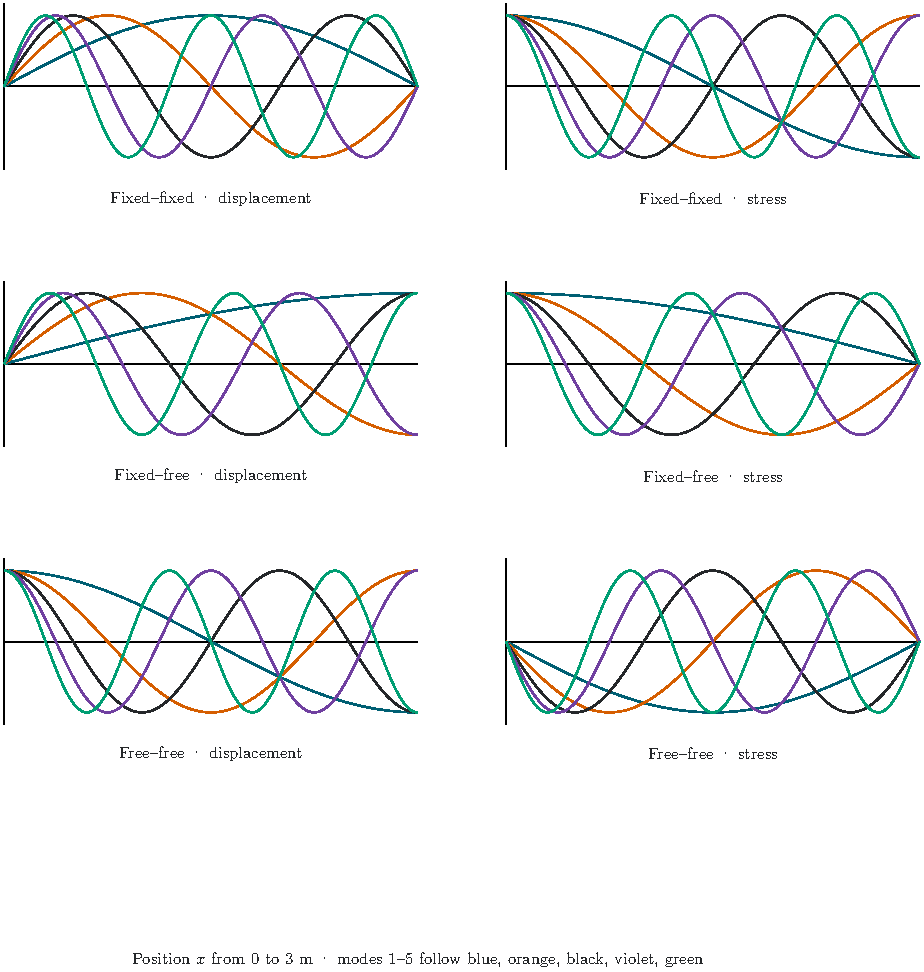
\includegraphics[width=0.95\linewidth]{figures/generated/solutions/C7.pdf}
\caption{Unit-peak displacement and stress modes for each boundary condition.}
\end{figure}

The MATLAB script integrates \(\int_0^L U_iU_j\,dx\) on the requested 1000-point grid. The diagonal terms equal one and the off-diagonal terms equal zero to numerical precision. Fixed--free frequencies are odd quarter-wave multiples, while fixed--fixed and free--free elastic frequencies coincide. The stress modes vanish at free ends and the displacement modes vanish at fixed ends. These boundary conditions and mode families agree with the slender-bar sections of the course notes.
\lstinputlisting[style=hwmatlab]{matlab/C7.m}
